\documentclass[11pt]{article}

%%%%%%%%%%%%%%Include Packages%%%%%%%%%%%%%%%%%%%%%%%%%%
\usepackage{xcolor}
\usepackage{mathtools}
\usepackage[a4paper, total={6in, 8in}, margin=1.25in]{geometry}
\usepackage{amsmath}
\usepackage{amssymb}
\usepackage{paralist}
\usepackage{rsfso}
\usepackage{amsthm}
\usepackage{wasysym}
\usepackage[inline]{enumitem}   
\usepackage{hyperref}
\usepackage{tocloft}
\usepackage{titlesec}
\usepackage{colortbl}
\usepackage{wrapfig}
\usepackage{pdfpages}
%%%%%%%%%%%%%%%%%%%%%%%%%%%%%%%%%%%%%%%%%%%%%%%%%%%%%%%%



\begin{document}
%\begin{wrapfigure}[9]{r}{0.3\textwidth}
%  \begin{center}
%  \vspace{-15pt}
%    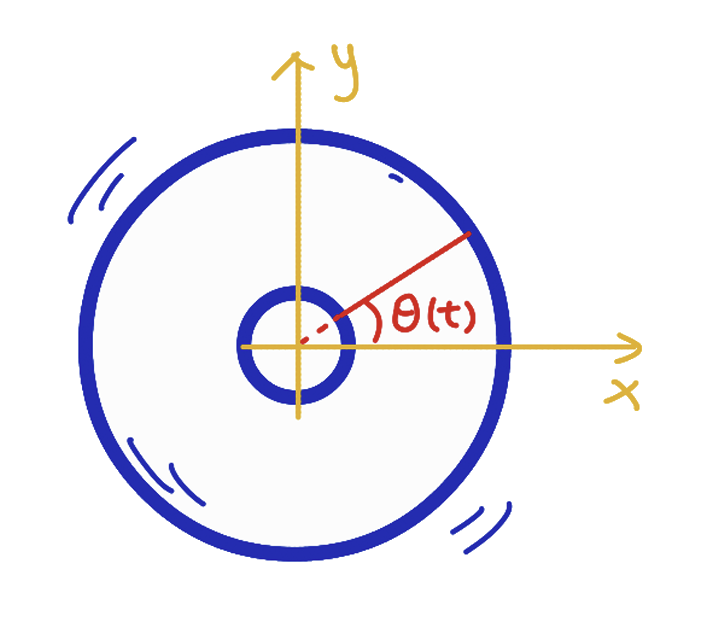
\includegraphics[scale=0.19]{disk}
%  \end{center}
%\end{wrapfigure}
\Large \noindent \textbf{Notes on Precession }\\
\normalsize
Jinyan Miao, Department of Physics and Astronomy, UCLA\\
\noindent\rule{8cm}{0.4pt}\\
\subsection{Larmor precession}
In classical E$\&$M theory, the magnetic moment $\vec{\mu}$ of some object in an external magnetic field $\vec{B}$ is defined via
\begin{align*}
\vec{\tau} = \vec{\mu} \times \vec{B}\,,\tag{*}
\end{align*}
where $\vec{\tau}$ is the torque experienced by the object due to being placed in $\vec{B}$. In intro-level physics, (*) is usually derived from Lorentz force law applied on a current loop in magnetic field. \\

For a torque $\vec{\tau}$, classically it is understood as the rate of change in angular momentum $\vec{L}$ of the object in which $\vec{\tau}$ is applied on, 
\begin{align*}
\vec{\tau} = \frac{d\vec{L}}{dt}\,.
\end{align*}
If one associates the magnetic moment $\vec{\mu}$ of the object to its angular momentum $\vec{L}$ (such as spin of an electron, as a quantum mechanical object) via
\begin{align*}
\vec{\mu} =\gamma\vec{L}\,,
\end{align*}
where $\gamma$ is a constant called the gyromagnetic ratio, then we obtain a precession equation 
\begin{align*}
\frac{d\vec{L}}{dt} = \gamma \vec{L}\times \vec{B}\,.
\end{align*}
Such a precession is known as the Larmor precession, which describes the precession of $\vec{\mu}$ around the external magnetic field lines. \\

However, for a classical macroscopic magnet bar (a large piece of magnet bar that has south and north ``poles"), such Larmor precession cannot be observed (such as a compass subjected to the Earth's magnetic field). The magnet bar will experience the torque given by (*) and align itself with the external field, instead of precessing around the field lines. One interpretation of this effect is via the use of damping effect (see the section for Landau-Lifshitz-Gilbert equation), or one can explain by arguing that $\vec{L}$ is small for bar magnet. \footnote{Some interesting point of views can be found here: \url{https://www.physicsforums.com/threads/a-magnetic-dipole-in-a-magnetic-field.864607/}.}\\

In the description of quantum mechanics, Larmor precession is again the precession of a particle's angular momentum around an applied magnetic field. Consider the magnetic moment $\hat{\vec{\mu}}$ of an object in a uniform field $\vec{B}$. We will write the Hamiltonian in the form 
\begin{align*}
H = -\hat{\vec{\mu}}\cdot \vec{B}\,,
\end{align*}
such that, for instance, if $\hat{\vec{\mu}} = \gamma \hbar\hat{\vec{S}}$ with $\gamma$ being the gyromagnetic ratio and $\hbar\hat{\vec{S}}$ being the spin (angular momentum) of the particle, we have
\begin{align*}
\hat{H} = -\gamma \hbar\hat{\vec{S}}\cdot \vec{B}\,.
\end{align*} 
Then we can use Heisenberg equation of motion to compute
\begin{align*}
\frac{d}{dt}(\hbar\hat{\vec{S}}) = \frac{i}{\hbar}[\hat{H}\,,\, \hbar\hat{\vec{S}}] = \gamma\hbar\hat{\vec{S}}\times \vec{B}\,.
\end{align*}
This recovers (*) in the classical case, and we see that the spin does not tip into $\vec{B}$, it precesses around $\vec{B}$ at a fixed angle in the absence of relaxation. The Larmor angular frequency is then defined as
\begin{align*}
\vec{\omega} = \gamma\vec{B}\,,
\end{align*}
from which we can rewrite the Hamiltonian,
\begin{align*}
\hat{H} = -\hbar \hat{\vec{S}} \cdot \vec{\omega}\,.
\end{align*}

\end{document}


